%\vspace{10pt}
\section{Modeling of the Cross-Point Memory}\label{sec:model}

%In this section, we present a detailed mathematical model for cross-point
%arrays. By using this model, along with specific parameters and edge
%conditions, the reliability, energy consumption, and area overheads of
%different read/write schemes can be easily evaluated.

%\subsection{Basic model of Cross-Point Memory}
The basic circuit model of an $M$ by $N$ cross-point ReRAM array is shown
in Figure~\ref{fig:modeling}. The model is built upon Kirchhoff's Current
Law (KCL) and its validity can be guaranteed by deductions from the basic
circuit theory. The horizontal lines are wordlines and vertical lines
represent bitlines. The ReRAM cells are located at each cross-point of
wordline and bitlines. The resistance of the ReRAM cell at the cross-point
of $i^{th}$ wordline and $j^{th}$ bitline is represented by $R_{i,j}$. We
assume the resistance of the wire connecting two cross-points to be
$R_{line}$. The input resistance of each wordline and bitline is $R_v$ and
the resistance of sense amplifier is $R_s$. In order to set up the KCL
equations, the voltage at each cross-point is indicated as $V_{i,j}$ for
wordline and $V'_{i,j}$ for bitline. A detailed cross-point is also shown
in Figure~\ref{fig:modeling}(b). The input voltage for the $i^{th}$
wordline is $V_{Wi}$ and the $i^{th}$ bitline is $V_{Bi}$. In the case
where a wordline takes input from both the sides, the voltage at the other
end of the $i^{th}$ wordline is represented as $V'_{Wi}$.
%Finally, the voltage at the sense amplifier is $V'_{Bi}$ during the read operation.
%YOU MIGHT WANT TO CHANGE THE ABOVE PARA INTO A TABLE

\begin{figure}%[!hb]
\centering
  % Requires \usepackage{graphicx}
  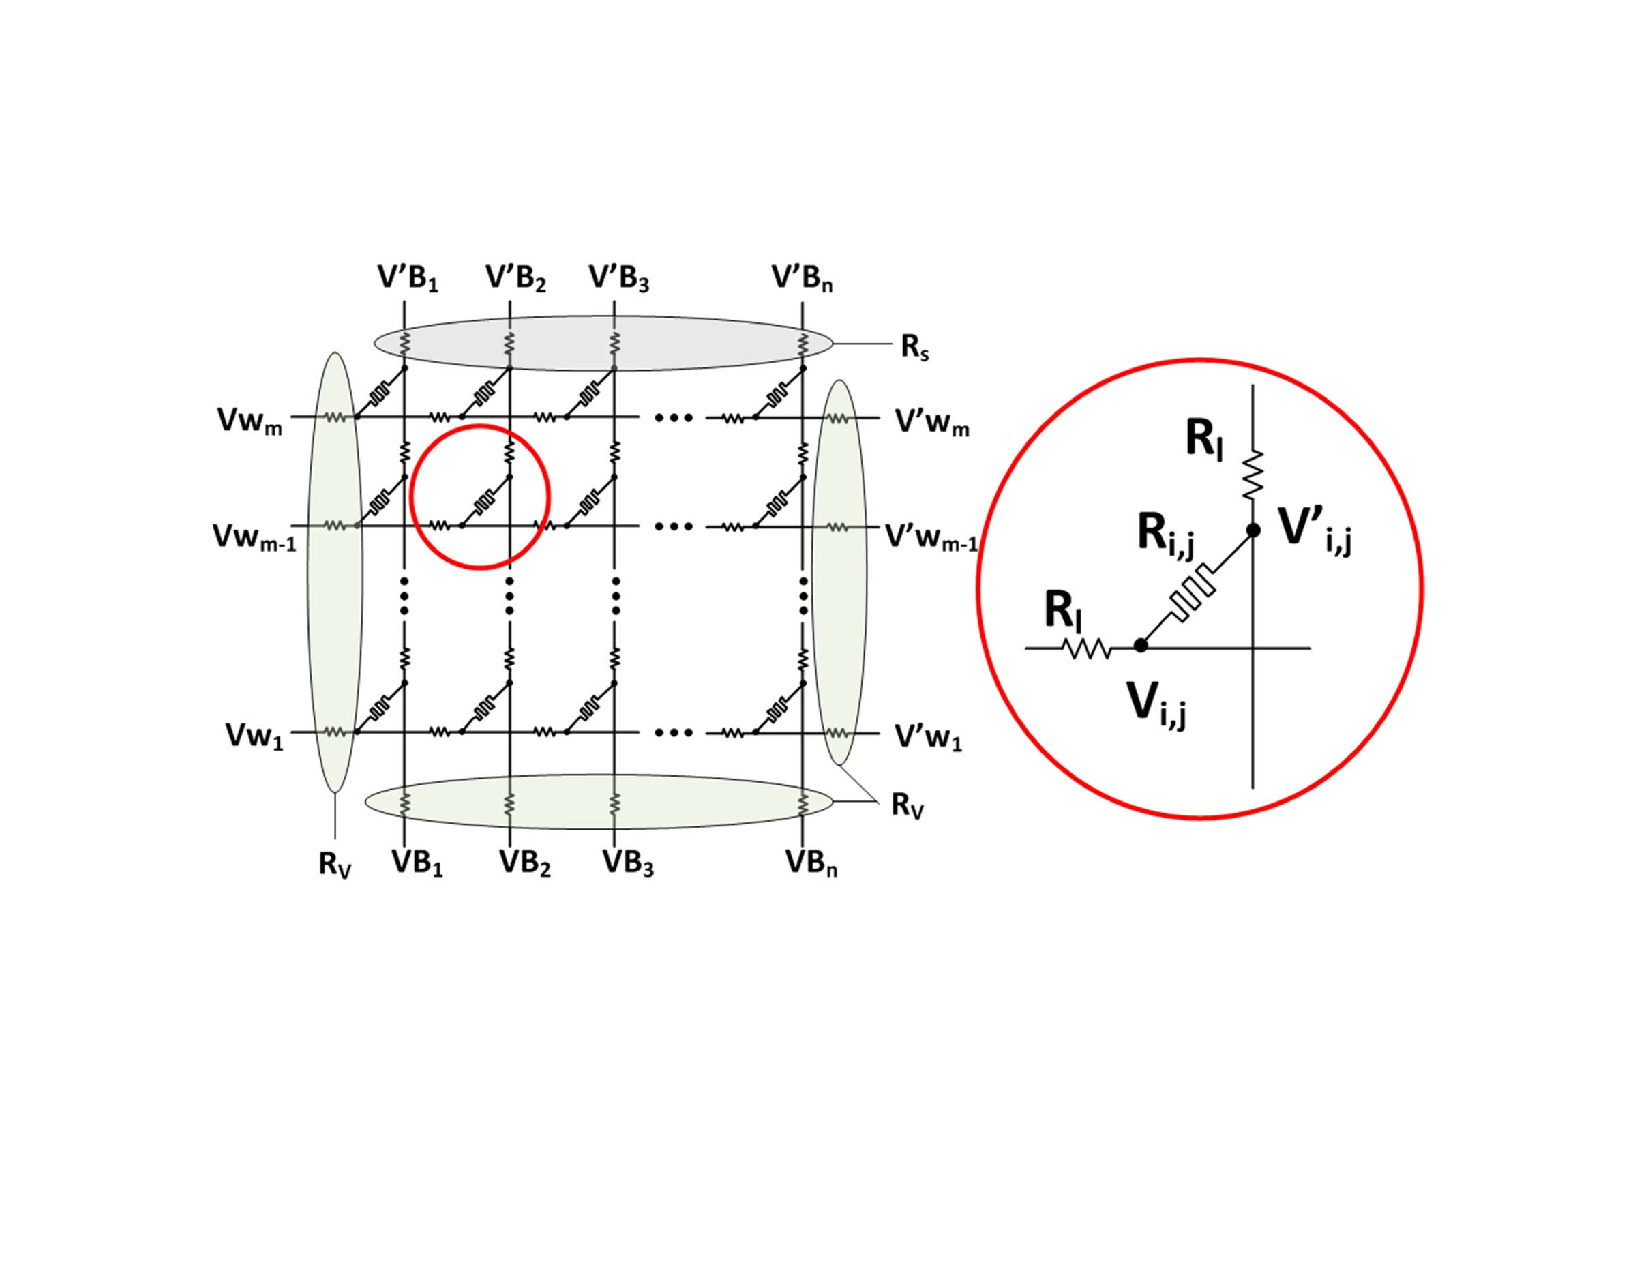
\includegraphics[width=0.45\textwidth]{./figures/model_f.pdf}\\
  \caption{The basic model of typical cross-point array.}\label{fig:modeling}
  \vspace{-12pt}
\end{figure}

%\subsection{Mathematical Model of a Cross-Point Array}
Based on this model, the current equations for each cross-point can be set
following KCL: $ {\Sigma}_{I=1}^kI_k=0.$ All of the cross-points have
similar structure with no more than three current branches and therefore
it is very easy to set up the KCL equations for each cross-point. However,
we should treat the cross-points at the edges of the array specifically
because KCL equations for these cross-points vary with different
write/read schemes. For example, the unselected wordline for write
operation can be either half biased or left floating. Thus, the edge
conditions should be adjusted according to each write/read scheme. In
particular, all of the cross-points in an array can be classified into
three major categories: \emph{normal point}, \emph{activated point} and
\emph{floating point}.

The normal points are located inside the memory array. In other words, for
all of the nodes with $1<i<m$ and $1<j<n$, the KCL equations take the form
of
\begin{equation}\label{equ:KCL1}
R_l^{-1}V_{i,j-1} -(2R_l^{-1}+R_{i,j}^{-1})V_{i,j}+ R_l^{-1}V_{i,j+1}+R_{i,j}^{-1}V'_{i,j}=0,
\end{equation}
for the node at wordline layer and
\begin{equation}\label{equ:KCL2}
R_l^{-1}V'_{i-1,j} -(2R_l^{-1}+R_{i,j}^{-1})V'_{i,j}+ R_l^{-1}V'_{i+1,j}+R_{i,j}^{-1}V_{i,j}=0,
\end{equation}
for the node at bitline layer.

The activated point and floating point represent the nodes at the edge of
cross-point array with different conditions: an edge point, which is
directly connected to the voltage input or to the ground, can be
considered as an activated point. Otherwise, it is a floating point. For
example, consider the point located at the intersection of $i^{th}$
wordline and $1^{st}$ bitline. If the $i^{th}$ wordline is activated by an
input voltage of $V_{Wi}$, this cross-point is an activated point, and the
KCL equation for this point is:
\begin{equation}\label{equ:KCL3}
-(R_v^{-1}+R_l^{-1}+R_{i,1}^{-1})V_{i,1}+ R_l^{-1}V_{i,2}+R_{i,1}^{-1}V'_{i,1}=-R_v^{-1}V_{Wi}.
\end{equation}
Otherwise, it is floating and its KCL equation is
\begin{equation}\label{equ:KCL4}
-(R_l^{-1}+R_{i,1}^{-1})V_{i,1}+ R_l^{-1}V_{i,2}+R_{i,1}^{-1}V'_{i,1}=0.
\end{equation}

For clarity, a ${2mn\times 1}$ vector ${V}$ is defined to represent all of the variables in the KCL equations:
\begin{equation}\label{equ:V1}
{V}=[{V_1}^T,{V_2}^T...{V_m}^T,{V'_1}^T,{V'_2}^T...{V'_m}^T]^T,
\end{equation}
where,
%\begin{equation}\label{equ:V2}
%{V_i} = [V_{i,1},V_{i,2}...V_{i,n}]^T,\\
%\end{equation}
%\begin{equation}\label{equ:V3}
%{V'_i} = [V'_{i,1},V'_{i,2}...V'_{i,n}]^T,
%\end{equation}
\begin{equation}\label{equ:V2}
{V_i} = [V_{i,1},V_{i,2}...V_{i,n}]^T,~~{V'_i} = [V'_{i,1},V'_{i,2}...V'_{i,n}]^T,
\end{equation}
for $i=1,2...m$. Then all of the KCL equations can be considered as a
system of linear equations, which has the form
\begin{equation}\label{equ:matrix}
A\cdot V = C.
\end{equation}
$A$ is a ${2mn\times{2mn}}$ coefficient matrix, which is determined by
Equations(\ref{equ:KCL1})-(\ref{equ:KCL4}). $C$ is a ${2mn\times{1}}$
vector, containing the constant terms of these equations. As shown, all of
the KCL equations have simple structure and are similar to each
other. Therefore, the linear equation system has a relatively fixed format
and simple structure, making it easy to establish and adjust the
coefficients and constants according to different design schemes. Besides,
due to the simplicity of the KCL equation, $A$ is populated primarily with
zeros and can be saved as a sparse matrix, which will further reduce the
storage cost during the computation.

To validate our analytical model, we compared the results with the HSPICE
simulations using simple a resistor model in cross-point memory arrays. DC
analysis was performed by HSPICE which solved the voltage of every node in
the array. The results of eight cross-point arrays with different array
size and specific data pattern are shown in Figure ??, the voltage drop on
the selected cell derived by our analytical model are consistent with the
HSPICE simulation results.

%
%The characteristics of the linear system can be summarized as:
%\begin{enumerate}
%  \item
%  As shown in Equation~(\ref{equ:blockedmatrix}), the coefficient matrix $A$ can be further partitioned into 4 smaller subblocks :
%    \begin{equation}\label{equ:blockedmatrix}
%        \mathbf{A} = \left[
%        \begin{array}{cc}
%            A1 & A2  \\
%            A3 & A4  \\
%        \end{array} \right].
%    \end{equation}
%All of these subblocks have the same size of $m\times n$. Subblock
%$A2$ and $A3$ are diagonal matrixes and have the value of: $A2_{i,i} =
%A3_{i,i} = R_{i,i}^{-1}$. $A2$ and $A3$ do not change their values
%with different schemas. However, $A1$ and $A4$ are a little more
%complex than $A2$ and $A3$. $A1$ is a tridiagonal matrix and has
%nonzero elements only in the main diagonal, and the first line below
%and above the diagonal. Similarly, $A_4$ is a special tridiagonal
%matrix, which has nonzero elements in the main diagonal, and the
%$n^{th}$ line below and above the diagonal, where $n$ is the number of
%bitline in the cross-point model. The value of the elements in $A1$
%and $A4$ can be easily derived from Equation (\ref{equ:KCL1}) and
%(\ref{equ:KCL2}). However, the edge condition varies with different
%program schemes. Therefore, the coefficients related to the edge
%condition should be set according to the program schemes. Clearly, the
%four edges shown in Figure~\ref{fig:modeling} correspond to different
%coefficients in $A1$ and $A4$. Due to the space limitations, we
%consider the nodes at the left edge of the array as an example. A
%similar procedure can be followed to initiate the coefficients of
%other edge. The coefficients of nodes at the left edge of the array
%($V_{i,1}$) can be set as:
%
%    \begin{equation}
%    A1(k,k) = \left\{
%    \begin{array}{ll}
%    -(R_l^{-1}+R_{i,1}^{-1})   & \text{if } floating\\
%    -(R_v^{-1}+R_l^{-1}+R_{i,1}^{-1})& \text{if } activated
%    \end{array} \right.
%    \end{equation}
%    where $k=(n-1)i+1$ for $i=1,2...m$.
%
%  \item The constant terms $C$ is a $2mn{\times}1$ vector. Equation(\ref{equ:KCL1})-(\ref{equ:KCL4}) show that only KCL equations of the activated points have constant terms. Therefore, only the following elements in $C$ may have non-zero value: $C((i-1)n+1)$, $C(in)$, $C(mn+i)$ and $C((2m-1)n+i)$ for $i=1,2...m$, corresponding to the nodes at the four edges respectively. Likewise, as an example, we consider nodes $V_{i,1}$. The constant corresponding to these nodes can be defined as:
%    \begin{equation}
%    C((i-1)n+1) = \left\{
%    \begin{array}{ll}
%    0   & \text{if } floating\\
%    -R_v^{-1}V_{Wi}& \text{if } activated
%    \end{array} \right.
%    \end{equation}
%\end{enumerate}
Thus, with parameters such as the resistance of ReRAM cells, the
resistance of interconnect wires, program voltages, and write/read
schemes, voltages at various cross points can be obtained by solving the
system of linear equations. With detailed voltage values,
$V_{2mn{\times}1}$, we can analyze the array at a fine granularity. These
values are also critical to evaluate reliability, energy consumption,
driven current density, and area overheads of a cross-point array.
